
%%%%%%%%%%%%%%%%%% PREAMBULE %%%%%%%%%%%%%%%%%%

\documentclass[aspectratio=169,utf8]{beamer}
%\documentclass[aspectratio=169,handout]{beamer}

\usetheme{Boadilla}
%\usecolortheme{seahorse}
\usecolortheme[RGB={245,66,24}]{structure}
\useoutertheme{infolines}

% packages
\usepackage{amsfonts,amsmath,amssymb,amsthm}
\usepackage[utf8]{inputenc}
\usepackage[T1]{fontenc}
\usepackage{lmodern}

\usepackage[francais]{babel}
\usepackage{fancybox}
\usepackage{graphicx}

\usepackage{float}
\usepackage{xfrac}

%\usepackage[usenames, x11names]{xcolor}
\usepackage{tikz}
\usepackage{pgfplots}
\usepackage{datetime}



%-----  Package unités -----
\usepackage{siunitx}
\sisetup{locale = FR,detect-all,per-mode = symbol}

%\usepackage{mathptmx}
%\usepackage{fouriernc}
%\usepackage{newcent}
%\usepackage[mathcal,mathbf]{euler}

%\usepackage{palatino}
%\usepackage{newcent}
% \usepackage[mathcal,mathbf]{euler}



% \usepackage{hyperref}
% \hypersetup{colorlinks=true, linkcolor=blue, urlcolor=blue,
% pdftitle={Exo7 - Exercices de mathématiques}, pdfauthor={Exo7}}


%section
% \usepackage{sectsty}
% \allsectionsfont{\bf}
%\sectionfont{\color{Tomato3}\upshape\selectfont}
%\subsectionfont{\color{Tomato4}\upshape\selectfont}

%----- Ensembles : entiers, reels, complexes -----
\newcommand{\Nn}{\mathbb{N}} \newcommand{\N}{\mathbb{N}}
\newcommand{\Zz}{\mathbb{Z}} \newcommand{\Z}{\mathbb{Z}}
\newcommand{\Qq}{\mathbb{Q}} \newcommand{\Q}{\mathbb{Q}}
\newcommand{\Rr}{\mathbb{R}} \newcommand{\R}{\mathbb{R}}
\newcommand{\Cc}{\mathbb{C}} 
\newcommand{\Kk}{\mathbb{K}} \newcommand{\K}{\mathbb{K}}

%----- Modifications de symboles -----
\renewcommand{\epsilon}{\varepsilon}
\renewcommand{\Re}{\mathop{\text{Re}}\nolimits}
\renewcommand{\Im}{\mathop{\text{Im}}\nolimits}
%\newcommand{\llbracket}{\left[\kern-0.15em\left[}
%\newcommand{\rrbracket}{\right]\kern-0.15em\right]}

\renewcommand{\ge}{\geqslant}
\renewcommand{\geq}{\geqslant}
\renewcommand{\le}{\leqslant}
\renewcommand{\leq}{\leqslant}
\renewcommand{\epsilon}{\varepsilon}

%----- Fonctions usuelles -----
\newcommand{\ch}{\mathop{\text{ch}}\nolimits}
\newcommand{\sh}{\mathop{\text{sh}}\nolimits}
\renewcommand{\tanh}{\mathop{\text{th}}\nolimits}
\newcommand{\cotan}{\mathop{\text{cotan}}\nolimits}
\newcommand{\Arcsin}{\mathop{\text{arcsin}}\nolimits}
\newcommand{\Arccos}{\mathop{\text{arccos}}\nolimits}
\newcommand{\Arctan}{\mathop{\text{arctan}}\nolimits}
\newcommand{\Argsh}{\mathop{\text{argsh}}\nolimits}
\newcommand{\Argch}{\mathop{\text{argch}}\nolimits}
\newcommand{\Argth}{\mathop{\text{argth}}\nolimits}
\newcommand{\pgcd}{\mathop{\text{pgcd}}\nolimits} 


%----- Commandes divers ------
\newcommand{\ii}{\mathrm{i}}
\newcommand{\dd}{\text{d}}
\newcommand{\id}{\mathop{\text{id}}\nolimits}
\newcommand{\Ker}{\mathop{\text{Ker}}\nolimits}
\newcommand{\Card}{\mathop{\text{Card}}\nolimits}
\newcommand{\Vect}{\mathop{\text{Vect}}\nolimits}
\newcommand{\Mat}{\mathop{\text{Mat}}\nolimits}
\newcommand{\rg}{\mathop{\text{rg}}\nolimits}
\newcommand{\tr}{\mathop{\text{tr}}\nolimits}


%----- Structure des exercices ------

\newtheoremstyle{styleexo}% name
{2ex}% Space above
{3ex}% Space below
{}% Body font
{}% Indent amount 1
{\bfseries} % Theorem head font
{}% Punctuation after theorem head
{\newline}% Space after theorem head 2
{}% Theorem head spec (can be left empty, meaning ‘normal’)

%\theoremstyle{styleexo}
\newtheorem{exo}{Exercice}
\newtheorem{ind}{Indications}
\newtheorem{cor}{Correction}


\newcommand{\exercice}[1]{} \newcommand{\finexercice}{}
%\newcommand{\exercice}[1]{{\tiny\texttt{#1}}\vspace{-2ex}} % pour afficher le numero absolu, l'auteur...
\newcommand{\enonce}{\begin{exo}} \newcommand{\finenonce}{\end{exo}}
\newcommand{\indication}{\begin{ind}} \newcommand{\finindication}{\end{ind}}
\newcommand{\correction}{\begin{cor}} \newcommand{\fincorrection}{\end{cor}}

\newcommand{\noindication}{\stepcounter{ind}}
\newcommand{\nocorrection}{\stepcounter{cor}}

\newcommand{\fiche}[1]{} \newcommand{\finfiche}{}
\newcommand{\titre}[1]{\centerline{\large \bf #1}}
\newcommand{\addcommand}[1]{}
\newcommand{\video}[1]{}

% Marge
\newcommand{\mymargin}[1]{\marginpar{{\small #1}}}

\def\noqed{\renewcommand{\qedsymbol}{}}


%----- Presentation ------
\setlength{\parindent}{0cm}

%\newcommand{\ExoSept}{\href{http://exo7.emath.fr}{\textbf{\textsf{Exo7}}}}

\definecolor{myred}{rgb}{0.93,0.26,0}
\definecolor{myorange}{rgb}{0.97,0.58,0}
\definecolor{myyellow}{rgb}{1,0.86,0}

\newcommand{\LogoExoSept}[1]{  % input : echelle
{\usefont{U}{cmss}{bx}{n}
\begin{tikzpicture}[scale=0.1*#1,transform shape]
  \fill[color=myorange] (0,0)--(4,0)--(4,-4)--(0,-4)--cycle;
  \fill[color=myred] (0,0)--(0,3)--(-3,3)--(-3,0)--cycle;
  \fill[color=myyellow] (4,0)--(7,4)--(3,7)--(0,3)--cycle;
  \node[scale=5] at (3.5,3.5) {Exo7};
\end{tikzpicture}}
}


\newcommand{\debutmontitre}{
  \author{} \date{} 
  \thispagestyle{empty}
  \hspace*{-10ex}
  \begin{minipage}{\textwidth}
    \titlepage  
  \vspace*{-2.5cm}
  \begin{center}
    \LogoExoSept{2.5}
  \end{center}
  \end{minipage}

  \vspace*{-0cm}
  
  % Astuce pour que le background ne soit pas discrétisé lors de la conversion pdf -> png
\begin{tikzpicture}
        \fill[opacity=0,green!60!black] (0,0)--++(0,0)--++(0,0)--++(0,0)--cycle; 
\end{tikzpicture}

% toc S'affiche trop tot :
% \tableofcontents[hideallsubsections, pausesections]
}

\newcommand{\finmontitre}{
  \end{frame}
  \setcounter{framenumber}{0}
} % ne marche pas pour une raison obscure

%----- Commandes supplementaires ------

% \usepackage[landscape]{geometry}
% \geometry{top=1cm, bottom=3cm, left=2cm, right=10cm, marginparsep=1cm
% }
% \usepackage[a4paper]{geometry}
% \geometry{top=2cm, bottom=2cm, left=2cm, right=2cm, marginparsep=1cm
% }

%\usepackage{standalone}


% New command Arnaud -- november 2011
\setbeamersize{text margin left=24ex}
% si vous modifier cette valeur il faut aussi
% modifier le decalage du titre pour compenser
% (ex : ici =+10ex, titre =-5ex

\theoremstyle{definition}
%\newtheorem{proposition}{Proposition}
%\newtheorem{exemple}{Exemple}
%\newtheorem{theoreme}{Théorème}
%\newtheorem{lemme}{Lemme}
%\newtheorem{corollaire}{Corollaire}
%\newtheorem*{remarque*}{Remarque}
%\newtheorem*{miniexercice}{Mini-exercices}
%\newtheorem{definition}{Définition}

% Commande tikz
\usetikzlibrary{calc}
\usetikzlibrary{patterns,arrows}
\usetikzlibrary{matrix}
\usetikzlibrary{fadings} 

%definition d'un terme
\newcommand{\defi}[1]{{\color{myorange}\textbf{\emph{#1}}}}
\newcommand{\evidence}[1]{{\color{blue}\textbf{\emph{#1}}}}
\newcommand{\assertion}[1]{\emph{\og#1\fg}}  % pour chapitre logique
%\renewcommand{\contentsname}{Sommaire}
\renewcommand{\contentsname}{}
\setcounter{tocdepth}{2}



%------ Figures ------

\def\myscale{1} % par défaut 
\newcommand{\myfigure}[2]{  % entrée : echelle, fichier figure
\def\myscale{#1}
\begin{center}
\footnotesize
{#2}
\end{center}}


%------ Encadrement ------

\usepackage{fancybox}


\newcommand{\mybox}[1]{
\setlength{\fboxsep}{7pt}
\begin{center}
\shadowbox{#1}
\end{center}}

\newcommand{\myboxinline}[1]{
\setlength{\fboxsep}{5pt}
\raisebox{-10pt}{
\shadowbox{#1}
}
}

%--------------- Commande beamer---------------
\newcommand{\beameronly}[1]{#1} % permet de mettre des pause dans beamer pas dans poly


\setbeamertemplate{navigation symbols}{}
\setbeamertemplate{footline}  % tiré du fichier beamerouterinfolines.sty
{
  \leavevmode%
  \hbox{%
  \begin{beamercolorbox}[wd=.333333\paperwidth,ht=2.25ex,dp=1ex,center]{author in head/foot}%
    % \usebeamerfont{author in head/foot}\insertshortauthor%~~(\insertshortinstitute)
    \usebeamerfont{section in head/foot}{\bf\insertshorttitle}
  \end{beamercolorbox}%
  \begin{beamercolorbox}[wd=.333333\paperwidth,ht=2.25ex,dp=1ex,center]{title in head/foot}%
    \usebeamerfont{section in head/foot}{\bf\insertsectionhead}
  \end{beamercolorbox}%
  \begin{beamercolorbox}[wd=.333333\paperwidth,ht=2.25ex,dp=1ex,right]{date in head/foot}%
    % \usebeamerfont{date in head/foot}\insertshortdate{}\hspace*{2em}
    \insertframenumber{} / \inserttotalframenumber\hspace*{2ex} 
  \end{beamercolorbox}}%
  \vskip0pt%
}


\definecolor{mygrey}{rgb}{0.5,0.5,0.5}
\setlength{\parindent}{0cm}
%\DeclareTextFontCommand{\helvetica}{\fontfamily{phv}\selectfont}

% background beamer
\definecolor{couleurhaut}{rgb}{0.85,0.9,1}  % creme
\definecolor{couleurmilieu}{rgb}{1,1,1}  % vert pale
\definecolor{couleurbas}{rgb}{0.85,0.9,1}  % blanc
\setbeamertemplate{background canvas}[vertical shading]%
[top=couleurhaut,middle=couleurmilieu,midpoint=0.4,bottom=couleurbas] 
%[top=fondtitre!05,bottom=fondtitre!60]



\makeatletter
\setbeamertemplate{theorem begin}
{%
  \begin{\inserttheoremblockenv}
  {%
    \inserttheoremheadfont
    \inserttheoremname
    \inserttheoremnumber
    \ifx\inserttheoremaddition\@empty\else\ (\inserttheoremaddition)\fi%
    \inserttheorempunctuation
  }%
}
\setbeamertemplate{theorem end}{\end{\inserttheoremblockenv}}

\newenvironment{theoreme}[1][]{%
   \setbeamercolor{block title}{fg=structure,bg=structure!40}
   \setbeamercolor{block body}{fg=black,bg=structure!10}
   \begin{block}{{\bf Th\'eor\`eme }#1}
}{%
   \end{block}%
}


\newenvironment{proposition}[1][]{%
   \setbeamercolor{block title}{fg=structure,bg=structure!40}
   \setbeamercolor{block body}{fg=black,bg=structure!10}
   \begin{block}{{\bf Proposition }#1}
}{%
   \end{block}%
}

\newenvironment{corollaire}[1][]{%
   \setbeamercolor{block title}{fg=structure,bg=structure!40}
   \setbeamercolor{block body}{fg=black,bg=structure!10}
   \begin{block}{{\bf Corollaire }#1}
}{%
   \end{block}%
}

\newenvironment{mydefinition}[1][]{%
   \setbeamercolor{block title}{fg=structure,bg=structure!40}
   \setbeamercolor{block body}{fg=black,bg=structure!10}
   \begin{block}{{\bf Définition} #1}
}{%
   \end{block}%
}

\newenvironment{lemme}[0]{%
   \setbeamercolor{block title}{fg=structure,bg=structure!40}
   \setbeamercolor{block body}{fg=black,bg=structure!10}
   \begin{block}{\bf Lemme}
}{%
   \end{block}%
}

\newenvironment{remarque}[1][]{%
   \setbeamercolor{block title}{fg=black,bg=structure!20}
   \setbeamercolor{block body}{fg=black,bg=structure!5}
   \begin{block}{Remarque #1}
}{%
   \end{block}%
}


\newenvironment{exemple}[1][]{%
   \setbeamercolor{block title}{fg=black,bg=structure!20}
   \setbeamercolor{block body}{fg=black,bg=structure!5}
   \begin{block}{{\bf Exemple }#1}
}{%
   \end{block}%
}


\newenvironment{miniexercice}[0]{%
   \setbeamercolor{block title}{fg=structure,bg=structure!20}
   \setbeamercolor{block body}{fg=black,bg=structure!5}
   \begin{block}{Mini-exercices}
}{%
   \end{block}%
}


\newenvironment{tp}[0]{%
   \setbeamercolor{block title}{fg=structure,bg=structure!40}
   \setbeamercolor{block body}{fg=black,bg=structure!10}
   \begin{block}{\bf Travaux pratiques}
}{%
   \end{block}%
}
\newenvironment{exercicecours}[1][]{%
   \setbeamercolor{block title}{fg=structure,bg=structure!40}
   \setbeamercolor{block body}{fg=black,bg=structure!10}
   \begin{block}{{\bf Exercice }#1}
}{%
   \end{block}%
}
\newenvironment{algo}[1][]{%
   \setbeamercolor{block title}{fg=structure,bg=structure!40}
   \setbeamercolor{block body}{fg=black,bg=structure!10}
   \begin{block}{{\bf Algorithme}\hfill{\color{gray}\texttt{#1}}}
}{%
   \end{block}%
}


\setbeamertemplate{proof begin}{
   \setbeamercolor{block title}{fg=black,bg=structure!20}
   \setbeamercolor{block body}{fg=black,bg=structure!5}
   \begin{block}{{\footnotesize Démonstration}}
   \footnotesize
   \smallskip}
\setbeamertemplate{proof end}{%
   \end{block}}
\setbeamertemplate{qed symbol}{\openbox}


\makeatother
\usecolortheme[RGB={192,41,0}]{structure}

% Commande spécifique à ce chapitre
\newcommand{\Sage}{\texttt{Sage}}

\usepackage{textcomp}

\usepackage{listings}
\lstset{
  upquote=true,
  columns=flexible,
  keepspaces=true,
  basicstyle=\ttfamily,
  commentstyle=\color{gray},
  language=Python,
  showstringspaces=false,
  aboveskip=0em,  
  belowskip=0em,
  escapeinside=||,
  breaklines=true,
  postbreak=\raisebox{0ex}[0ex][0ex]{\qquad\ensuremath{\color{red}\hookrightarrow\space}},
}

\lstset{
  literate={é}{{\'e}}1
           {è}{{\`e}}1
           {à}{{\`a}}1
}

\newcommand{\codeinline}[1]{\lstinline!#1!}
   
%%%%%%%%%%%%%%%%%%%%%%%%%%%%%%%%%%%%%%%%%%%%%%%%%%%%%%%%%%%%%
%%%%%%%%%%%%%%%%%%%%%%%%%%%%%%%%%%%%%%%%%%%%%%%%%%%%%%%%%%%%%


\begin{document}


\title{{\bf Calcul formel}}
\subtitle{Algèbre linéaire}

\begin{frame}
  
  \debutmontitre

  \pause

{\footnotesize
\hfill
\setbeamercovered{transparent=50}
\begin{minipage}{0.6\textwidth}
  \begin{itemize}
    \item<3-> Opérations de base
    \item<4-> Réduction de Gauss, calcul de l'inverse
    \item<5-> Application linéaire, image, noyau
    \item<6-> Méthodes des moindres carrés
  \end{itemize}
\end{minipage}
}

\end{frame}

\setcounter{framenumber}{0}





%%%%%%%%%%%%%%%%%%%%%%%%%%%%%%%%%%%%%%%%%%%%%%%%%%%%%%%%%%%%%%%%
\section{Opérations de base}


\begin{frame}
\begin{tp}
Soient les matrices :
$$A = 
\begin{pmatrix}
1&2&3\\
-1&0&1\\
0&1&0\\ 
\end{pmatrix}
\quad
B = 
\begin{pmatrix}
2&-1&0\\
-1&0&1\\ 
\end{pmatrix}
\quad
u = \begin{pmatrix}1\\x\\x^2\end{pmatrix}
\quad
v = \begin{pmatrix}1\\0\\1\end{pmatrix}$$

\begin{enumerate}
  \item Calculer tous les produits possibles 
  à partir de $A,B,u,v$.
  
  \item Calculer $(A-I)^7$ et en extraire le coefficient 
  en position $(2,3)$.
  
  \item Calculer $A^{-1}$. Calculer la trace de $A^{-1}$
  (c'est-à-dire la somme des coefficients situés sur la diagonale).
\end{enumerate}
  
\end{tp}
\end{frame}




\begin{frame}[fragile]
\begin{enumerate}
  \item On définit une matrice $n$ lignes et $p$ colonnes par  \\
  \centerline{\codeinline{matrix(n,p,[ [ligne1],[ligne2],... ])}}
  
  \pause
  %\insertcode{formel/Algos/alglin-tex1.sage}{alglin.sage (1)} 
\begin{algo}[alglin.sage]
\begin{lstlisting}
A = matrix(3,3,[[1,2,3],[-1,0,1],[0,1,0]])
B = matrix(2,3,[[2,-1,0],[-1,0,1]])
u = matrix(3,1,[1,x,x^2])
v = matrix(3,1,[1,0,1])
\end{lstlisting}
\end{algo}
 
 
\bigskip
  \pause
  
  Produit $A\times B$ par \codeinline{A*B}
  \pause
  
  \begin{itemize}
    \item le nombre de colonnes de $A$ doit être égal au nombre de lignes de $B$
    \pause
    \item produits possibles sont : 
  $B\times A$, $A \times u$, $A \times v$,  $B \times u$, $B \times v$
  \end{itemize}

\end{enumerate}  
\end{frame}


\begin{frame} 
\begin{enumerate}
  \setcounter{enumi}{1}  
  \item 
  \begin{itemize}
    \item \codeinline{I = identity_matrix(3)}: matrice identité
    \smallskip
    \pause
    \item \codeinline{(A-I)^7} 
    \smallskip
    \pause
    \item $(A-I)^{7} = \begin{pmatrix}-16& -46&  11\\-25& -73& {\color<4->{red}153}\\32&  57& -137\\\end{pmatrix}$
    \smallskip
    \pause
    \item \codeinline{((A-I)^7)[1,2]} : coefficient en position $(2,3)$
  \end{itemize}
  
  
\bigskip 
  \pause
  \item 
  \begin{itemize}
    \item \codeinline{A^-1} (ou \codeinline{A.inverse()}) : inverse de \codeinline{A}
    \smallskip
    \pause
    \item $A^{-1} = \begin{pmatrix}\frac14&-\frac34&-\frac12\\0& 0& 1\\\frac14& \frac14&-\frac12\end{pmatrix}$
    \smallskip
    \pause
    \item la trace se calcule par une simple somme des éléments sur la diagonale principale
    \smallskip
    \pause
    \item \codeinline{sum( (A^-1)[i,i] for i in range(3) )}
    \smallskip
    \pause
    \item la trace de $A^{-1}$ vaut $-\frac14$
  \end{itemize}
  
\end{enumerate}
\end{frame}





\begin{frame}
\evidence{Remarques}

\begin{itemize}
  \item Coefficient \codeinline{A[i,j]} (\codeinline{i}
  pour les lignes, \codeinline{j} pour les colonnes)
\pause

  \item Pour \Sage\ les indices varient de $0$ à $n-1$
\pause
  
  \item  \codeinline{vector([x1,x2,...,xn])}
   \pause
   
  \item Exemple
  \begin{itemize}
    \item \codeinline{v = vector([1,2,3,4])}
    \pause
    
    \item \codeinline{L = matrix(v)} renvoie la matrice ligne correspondante
    \pause
    
    \item \codeinline{C = L.transpose()} renvoie la matrice colonne correspondante    
  \end{itemize} 
\end{itemize}


%\vspace*{-1ex}
%
%\begin{tp}
%Pour une matrice $A \in M_n(\Kk)$ inversible et des vecteurs colonnes $u,v$ à $n$ lignes
%%\in  \Kk^n$,
%on définit $\alpha \in \Kk$ par : 
%
%\vspace*{-2ex}
%$$\alpha  = 1 + v^T A^{-1} u.$$
%\vspace*{-3.5ex}
%
%La formule de Sherman-Morrison affirme que si $\alpha\neq0$ alors
%
%\vspace*{-2ex}
%$$\bigg(A+u v^T\bigg)^{-1} = A^{-1} - \frac{A^{-1}u v^T A^{-1}}{\alpha}$$
%\vspace*{-3.5ex}
%
%Prouver par le calcul formel cette formule pour les matrices de taille 
%$2\times2$ et $3\times 3$.
%\end{tp}
\end{frame}



%%%%%%%%%%%%%%%%%%%%%%%%%%%%%%%%%%%%%%%%%%%%%%%%%%%%%%%%%%%%%%%%
\section{Réduction de Gauss, calcul de l'inverse}

\begin{frame}
%Le but de cette section est est de mettre en \oe uvre la méthode de Gauss.
%Cette méthode est valable pour des systèmes linéaires (ou des matrices) de taille quelconque, 
%mais ici on se limite au calcul de l'inverse d'une matrice (qui est obligatoirement carrée). 
%N'hésitez pas à d'abord relire votre cours sur la méthode de Gauss.

\footnotesize

\begin{tp}
\begin{enumerate}
  \item Réaliser trois fonctions qui transforment une matrice en fonction des 
  opérations élémentaires sur les lignes :

\vspace*{-2ex}  

  \begin{itemize}
    \item \footnotesize$L_i \leftarrow c L_i$ avec $c \neq 0$ :
  on multiplie une ligne par un réel ;

    \item \footnotesize$L_i \leftarrow L_i+ c L_j$ :
  on ajoute à la ligne $L_i$ un multiple d'une autre ligne $L_j$ ;

    \item \footnotesize$L_i \leftrightarrow L_j$ : on échange deux lignes.
  \end{itemize}

 \vspace*{-2ex}
  
  \item À l'aide de ces transformations élémentaires, transformer par la méthode de Gauss
  une matrice inversible en une matrice échelonnée (c'est-à-dire ici, en partant d'une matrice carrée,
  obtenir une matrice triangulaire supérieure).
  
  \item Toujours à l'aide de ces transformations et de la méthode de Gauss, transformer 
  cette matrice échelonnée en une matrice échelonnée et réduite
  (c'est-à-dire ici, en partant d'une matrice inversible, obtenir l'identité).
  
  \item La méthode de Gauss permet de calculer l'inverse d'une matrice $A$ :

 \vspace*{-2ex}  
  
  \begin{itemize}
    \item \footnotesize Partant de $A$, on pose $B = I$ la matrice identité.
    \item \footnotesize Par la méthode de Gauss et des opérations élémentaires on transforme $A$ en 
    la matrice $I$. 
    \item \footnotesize On applique exactement les mêmes transformations à la matrice $B$.
    \item \footnotesize Lorsque $A$ s'est transformée en $I$ alors $B$ s'est transformée en $A^{-1}$.
  \end{itemize}
  
  \vspace*{-2ex} 
  
  Modifier légèrement vos deux fonctions (issues des questions 2. et 3.) afin 
  de calculer l'inverse d'une matrice.
\end{enumerate}
\end{tp}

\end{frame}




%%%%%%%%%%%%%%%%%%%%%%%%%%%%%%%%%%%%%%%%%%%%%%%%%%%%%%%%%%%%%%%%
\section{Application linéaire, image, noyau}

\begin{frame}
\begin{tp}
Soit $f : \Rr^3 \to \Rr^4$ l'application linéaire définie par
$$f : \begin{pmatrix}x\\y\\z\end{pmatrix}
\longmapsto 
\begin{pmatrix}
x+2z\\
5x+2y+2z\\
2x+y\\
x+y-2z
\end{pmatrix}.$$
\begin{enumerate}
  \item Expliciter la matrice $A$ de $f$ (dans les bases canoniques).
  Comment s'écrit alors l'application $f$ ?
    
  \item Calculer une base du noyau de $f$. L'application linéaire
  $f$ est-elle injective ?
  
  \item Calculer une base de l'image de $f$. L'application linéaire
  $f$ est-elle surjective ?
\end{enumerate}
\end{tp}
\end{frame}


\begin{frame}[fragile]

\begin{enumerate}
  \item 
  \begin{itemize}
    \item la matrice associée est $A = \left(\begin{smallmatrix}1&0&2\\5&2&2\\2&1&0\\1&1&-2\\\end{smallmatrix}\right)$
    \pause
    \item l'application linéaire $f$ étant alors définie par $X \mapsto Y = AX$
  \end{itemize}

  
%  Voici l'implémentation avec un exemple de calcul. 
%\insertcode{formel/Algos/matlin-tex1.sage}{matlin.sage (1)}    
%\begin{algo}[matlin.sage (1)]
%\begin{lstlisting}
%K = QQ
%A = matrix(K,4,3,[[1,0,2],[5,2,2],[2,1,0],[1,1,-2]])
%X = vector(K,[2,3,4])
%Y = A*X
%\end{lstlisting}
%\end{algo}
 \pause
  \item %et 3.
  \begin{itemize}
    \item \codeinline{right_kernel()} : le noyau
    \pause
    \item \codeinline{column_space()} : l'image
  \end{itemize}    
    
 \vspace*{-1ex} 
\pause

 % \insertcode{formel/Algos/matlin-tex2.sage}{matlin.sage (2)} 
 {\small   
\begin{algo}[matlin.sage]
\begin{lstlisting}
Ker = A.right_kernel()
Ker.basis()
Im = A.column_space()
Im.basis()
\end{lstlisting}
\end{algo}   
} 

\vspace*{-1ex}
\pause
  \begin{itemize}
    \item le noyau est un espace vectoriel de dimension $1$ dans $\Rr^3$ 
    \pause
    \item engendré par $\left(\begin{smallmatrix}2\\-4\\-1\end{smallmatrix}\right)$ 
    \pause
    \item l'application $f$ n'est pas injective
  \pause
    \item l'image est un espace vectoriel de dimension $2$ dans $\Rr^4$
    \pause
    
    \item une base est :
  $\left( 
  \left(\begin{smallmatrix}1\\1\\0\\ -1\end{smallmatrix}\right),
  \left(\begin{smallmatrix}0\\2\\ 1\\ 1\end{smallmatrix}\right)
  \right)$
   \pause
    \item $f$ n'est pas surjective
 
  
%    \item On peut tester si un vecteur donné est dans un sous-espace. Si on pose par exemple 
%      \codeinline{X = vector(K,[1,5,2,1])} alors le test \og \codeinline{X in Im} \fg{}
%      renvoie vrai. Ce vecteur est donc bien un élément de l'image de $f$. 
  \end{itemize}
 
\end{enumerate}


\end{frame}


%%%%%%%%%%%%%%%%%%%%%%%%%%%%%%%%%%%%%%%%%%%%%%%%%%%%%%%%%%%%%%%%
\section{Méthodes des moindres carrés}

\begin{frame}


\evidence{Méthodes des moindres carrés}

\pause
\begin{itemize}
  \item Résoudre un système linéaire avec plus d'équations que d'inconnues
  \pause
  \begin{itemize}
    \item pas de solution en général
    \pause
    \item solution approchée
    
  \end{itemize}
   \pause 
  \item $A \in M_{n,p}(\mathbb R)$ avec $n \ge p$
  \pause
  \item $X$ un vecteur inconnu de taille $p$
  \pause
  \item $B$ un vecteur de taille $n$
  \pause
  \item Pas de solution $X$ au système $AX=B$
  \pause
  \item \defi{Solution des moindres carrés} est un vecteur $X$ 
tel que $\| AX -B \|$ soit minimale
\pause
  \item Formule 
  \mybox{$X = (A^TA)^{-1} A^T B$}
\end{itemize}

\end{frame}


\begin{frame}

\begin{tp}

\begin{enumerate}
  \item \textbf{Régression linéaire.} 
  On considère les points $\big\{(-6,0), (-2,1), (1,2), (4,4), (6,4)\big\}$.
  Trouver la droite qui approche au mieux ces points (au sens des moindres carrés).
  
  \emph{Indications.} On pose $f(x) = a +bx$. On aimerait trouver $a,b \in \Rr$ tels que 
  $f(x_i)=y_i$ pour tous les points $(x_i,y_i)$ donnés. 
  Transformer le problème en un problème des moindres carrés : quel est le vecteur inconnu $X$ ?
  quelle est la matrice $A$ ? quel est le second membre $B$ ?
    
  \item \textbf{Interpolation polynomiale.} 
  Pour ces mêmes points, quel polynôme de degré $3$ approche 
  au mieux ces points (au sens des moindres carrés).
  
  \emph{Indication.} Cette fois $f(x) = a + bx + cx^2 + dx^3$.
  
  
%  \item 
\end{enumerate}
 
\end{tp}
\end{frame}

\begin{frame}
\begin{center}
    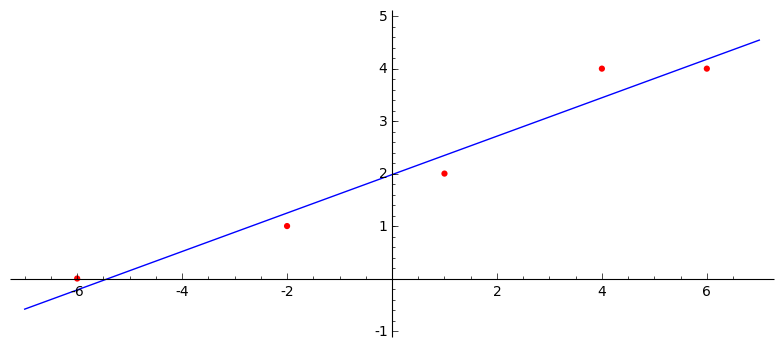
\includegraphics[scale=0.4]{figures/moindres_carres1}\\[8mm]
    \pause
    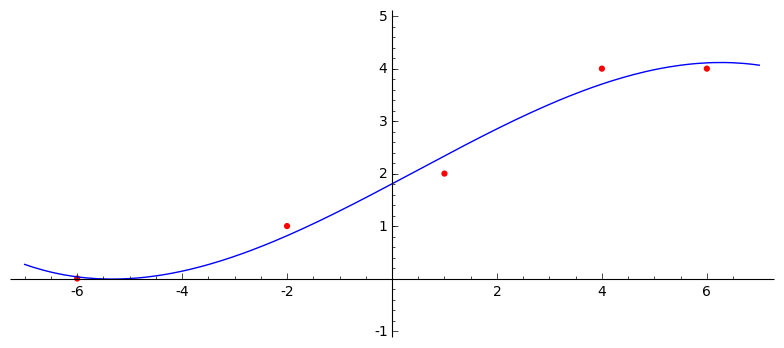
\includegraphics[scale=0.4]{figures/moindres_carres2}
\end{center} 
\end{frame}


\begin{frame}
  
\begin{enumerate}
  \item $\big\{(-6,0), (-2,1), (1,2), (4,4), (6,4)\big\}$
 \end{enumerate} 
 
\vspace*{-0.5ex}

\pause 
\begin{itemize}
  \item Points non alignés, pas de droite passant par tous les points
  \pause
  \item On cherche une droite $y = a +bx$ qui minimise (le carré de) la distance  
  entre les points et la droite
  \pause
  \item Posons $f(x) = a + bx$
  \pause
  \item Alors pour nos $n$ points $(x_i,y_i)$ donnés, on voudrait $f(x_i)=y_i$
\end{itemize}

\pause
  $
  \left\{ \!\!
  \begin{array}{c}
  f(x_1) = y_1 \\
  f(x_2) = y_2 \\
  \vdots  \\
  f(x_n) = y_n \\
  \end{array}
  \right.\!\!\!
  \pause\!\Leftrightarrow \!
  \left\{ \!\!
  \begin{array}{c}
  a +b x_1 = y_1 \\
  a +b x_2 = y_2 \\
  \vdots \\
  a +b x_n = y_n \\
  \end{array}
  \right.\!\!\!
  \pause\!\Leftrightarrow \!
  \left(\begin{smallmatrix}
  1 & x_1 \\
  1 & x_2 \\
  \vdots & \vdots \\
  1 & x_n \\  
  \end{smallmatrix}\right)\!\!
  \begin{pmatrix}
  a \\ b  
  \end{pmatrix}
  = 
  \left(\begin{smallmatrix}
  y_1\\
  y_2 \\
  \vdots \\
  y_n
  \end{smallmatrix}\right)
  \pause\!\Leftrightarrow\!
  AX = B
  $
  
 \pause
  
\begin{itemize}
  \item Solution approchée de $AX = B$, par la formule des moindres carrés
  \pause
  \item $X = \left(\begin{smallmatrix}a\\b\end{smallmatrix}\right) = (A^TA)^{-1} A^T B$
  \pause
  \item $y=a + bx$ équation de la droite des moindres carrés
\end{itemize}

\end{frame}



\begin{frame}[fragile]
  
 % \insertcode{formel/Algos/moindres_carres-tex1.sage}{moindres\_carres.sage (1)} 
\begin{algo}[moindres\_carres.sage]
\begin{lstlisting}
def moindres_carres(A,B):
    return (A.transpose()*A)^-1 * A.transpose() * B|\pause|

points = [(-6,0),(-2,1),(1,2),(4,4),(6,4)]|\pause|

A = matrix([ [1,p[0]] for p in points ])
B = vector(p[1] for p in points)
X = moindres_carres(A,B)
\end{lstlisting}
\end{algo} 

\pause

\begin{minipage}{0.29\textwidth}
$y = \frac{301}{152} + \frac{167}{456}x$
\end{minipage}
\begin{minipage}{0.49\textwidth}
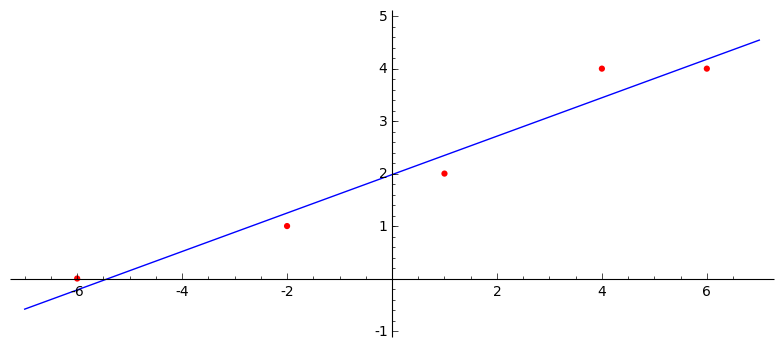
\includegraphics[scale=0.4]{figures/moindres_carres1}
\end{minipage}


    

\end{frame}


\begin{frame}
\begin{enumerate}
  \setcounter{enumi}{1}
  \item Même idée pour $f(x) = a + bx +c x^2 + dx^3$
   $$
  \left\{ 
  \begin{array}{rcl}
  f(x_1) &=& y_1 \\
  f(x_2) &=& y_2 \\
  \vdots && \vdots\\
  f(x_n) &=& y_n \\
  \end{array}
  \right.
  \quad
  \iff
  \quad
  \left\{ 
  \begin{array}{rcl}
  a +b x_1 + c x_1^2 + d x_1^3 &=& y_1 \\
  a +b x_2 + c x_2^2 + d x_2^3 &=& y_2 \\
  \vdots && \vdots\\
  a +b x_n + c x_n^2 + d x_n^3 &=& y_n \\
  \end{array}
  \right.
  $$
  $$
  \iff
  \quad 
  \begin{pmatrix}
  1 & x_1 & x_1^2 & x_1^3\\
  1 & x_2 & x_2^2 & x_2^3 \\
  \vdots & \vdots & \vdots & \vdots\\
  1 & x_n & x_n^2 & x_n^3  \\  
  \end{pmatrix}
  \begin{pmatrix}
  a \\ b \\ c \\ d
  \end{pmatrix}
  = 
  \begin{pmatrix}
  y_1\\
  y_2 \\
  \vdots \\
  y_n
  \end{pmatrix}
  \quad
  \iff
  \quad 
  AX = B
  $$ 
  
  %\insertcode{formel/Algos/moindres_carres-tex2.sage}{moindres\_carres.sage (2)} 
\begin{center}  
    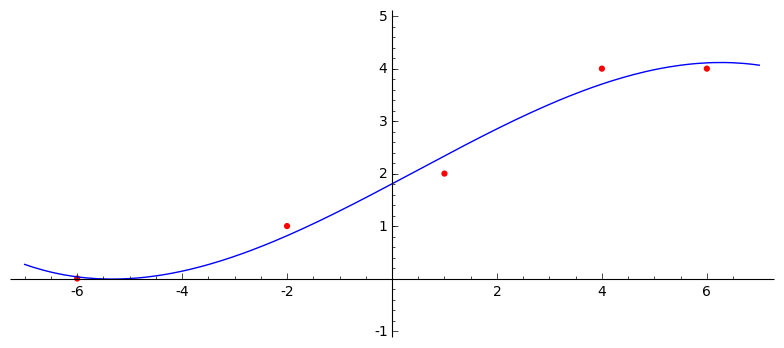
\includegraphics[scale=0.35]{figures/moindres_carres2}
\end{center}    
\end{enumerate}
\end{frame}


\end{document}
